\documentclass[conference,compsoc]{./IEEEtran/IEEEtran}

%% Configure which sections are included:
%\newcommand*{\OPTIONAL}{}


% *** CITATION PACKAGES ***
% IEEE Computer Society needs nocompress option
% requires cite.sty v4.0 or later (November 2003)
\usepackage[nocompress]{cite}

% *** ALIGNMENT PACKAGES ***
\usepackage{array}

% *** SUBFIGURE PACKAGES ***
\usepackage[caption=false,font=footnotesize,labelfont=sf,textfont=sf]{subfig}
% The latest version and documentation of subfig.sty can be obtained at:
% http://www.ctan.org/pkg/subfig

% correct bad hyphenation here
\hyphenation{op-tical net-works semi-conduc-tor}



\usepackage{hyperref}

\usepackage{graphicx}
\DeclareGraphicsExtensions{.png,.jpg,.pdf,.eps}

\usepackage{pgfplots}
\pgfplotsset{compat=1.9}


\begin{document}

\title{Peer-to-peer Browser Middleware\\
       for Communication and Consensus in an Unreliable Infrastructure}

\author{\IEEEauthorblockN{Joel Martin}
\IEEEauthorblockA{Department of Computer Science and Engineering\\
University of Texas at Arlington\\
Arlington, TX 76010\\
Email: joel@martintribe.org}
\and
\IEEEauthorblockN{David Levine}
\IEEEauthorblockA{Department of Computer Science and Engineering\\
University of Texas at Arlington\\
Arlington, TX 76010\\
Email: levine@cse.uta.edu}}

\maketitle

\begin{abstract}
We describe a browser-based peer-to-peer computing system/middleware that enables distributed consensus that is tolerant of degraded and/or unreliable centralized infrastructure. The system is composed of a JavaScript implementation of the Raft distributed consensus protocol (Raft.js) together with the WebRTC browser-to-browser communication protocol. The Raft over WebRTC middleware is used to build a demonstration chat application that guarantees a shared, consistent and linearized view of the chat history without relying on a single centralized server for communication. The correctness, robustness, performance, and scalability of the system is verified with a series of automated tests implemented using the SlimerJS browser automation tool.
\end{abstract}

\section{Use Case/Scenario}
Consider a scenario where emergency responders and volunteers are responding to a city-scale disaster in which utilities such as electrical power and communication systems are highly degraded or completely unavailable for an extended period. Emergency management officials have divided the city into zones each of which is assigned several dozen volunteers who systematically search the neighborhoods for people that are injured or in need and also for damaged infrastructure that needs to be repaired.

Responders and volunteers have access to a distributed disaster response datastore that is accessed and updated via a browser based application. Volunteers use their own mobile device and only require a browser with WebRTC capability to run the application. The application communicates over the cellular network (existing or provided by mobile emergency response cell stations) or mesh network (although this may also require additional installed software on mobile devices in order to support it). Once loaded and running, the application does not require any centralized servers or database system. The application uses the Raft distributed consensus protocol to maintain a distributed but consistent view of the datastore among all participating client nodes. Also, the distributed cluster is dynamic and allows nodes to join and leave over time without losing state or synchronization of the datastore.

The above capabilities are demonstrated using a distributed chat application implemented with the Raft over WebRTC middleware. This chat application uses direct browser-to-browser communication over WebRTC and maintains a consistent view of the chat history (exact same messages and ordering is seen by all nodes) and is fault tolerant (almost half the cluster nodes can fail simultaneously and the application will remain available without dataloss for the remaining clients).

\section{Background}

\subsection{Raft}

Raft is a new distributed consensus algorithm designed to be understandable and practical without sacrificing safety and correctness. The Raft algorithm implemented and described in this paper is based on Diego Ongaro's dissertation ``Consensus: Bridging Theory and Practice" \cite{raft_thesis:ongaro14}.

The Raft algorithm breaks the problem of consensus into three core sub-problems: leader election, log replication, and safety \cite[Section~3]{raft_thesis:ongaro14}. A full Raft system must also address: cluster membership changes \cite[Section~4]{raft_thesis:ongaro14}, log compaction \cite[Section~5]{raft_thesis:ongaro14}, and client interaction \cite[Section~6]{raft_thesis:ongaro14}. The Raft protocol is based on the concept of a distributed transaction log. Entries in the log represent a sequence of commands that will be applied to an internal state machine. If all members of the Raft cluster have the same log entries, then their state machine on each node will have exactly the same state. Each node of a Raft cluster can be in one of three states: follower, candidate, or leader. The responsibility of the leader is to accept new transaction log entries and then replicate these entries in the same order to all other members of the cluster. The leader is the only member of the cluster that may make changes to the transaction log. In order to maintain leadership, the leader sends heartbeat RPCs to all the followers in the cluster.  Followers that do not receive a heartbeat RPC within a certain time period become candidates and attempt to be elected by the other nodes as the new leader of the cluster \cite[p.~12]{raft_thesis:ongaro14}.

Raft leverages the replicated transaction log to accomplish live cluster membership changes. Membership changes are accomplished by adding or removing one Raft node at a time using special add/remove log entries. In order to keep the replicated transaction log from growing indefinitely, Raft nodes should periodically compact their logs. The simplest and most generic solution is often to provide some way of snapshotting the entire state machine (including the term and log index it represents) to disk at which point the all previously applied log entries can be discarded. Clients of the Raft cluster are able to interact with the distributed state machine by sending RPCs to the leader in order to add command entries to the transaction log. Clients first find the address of any node in the cluster and are then redirected to communicate directly with the leader. The Raft protocol also provides strict linearizable semantics for client commands/requests (reads and writes) for applications that require it.

\subsection{WebRTC}

WebRTC is a collection of browser APIs \cite{webrtc:feb2015} and network protocols \cite{draft-rtcweb-overview} that are currently being standardized by the W3C and IETF respectively. Collectively these APIs and protocols enable real-time peer-to-peer video, audio and data communication between browsers.

One of the challenges with browser-to-browser communication (and direct peer-to-peer communication in general) is that the browser is usually running behind a firewall in a private internet subnet. To establish a direct communication channel between browsers, WebRTC uses a mechanism called Interactive Connectivity Establishment (ICE) that is similar to the Session Initiation Protocol (SIP) commonly used for Voice-over-IP (VoIP) communication \cite{RFC5245:ice}. This process requires out-of-band exchange of information usually involving a third party server known as a signaling server. The signaling server may optionally provide other services such as higher level session management, HTTP serving of the web application, address book service, client presence/availability, etc.

\subsubsection{WebRTC APIs}

The WebRTC browser APIs enable JavaScript web applications to establish browser-to-browser network connectivity in order to perform real-time video, audio and data communication. These APIs are currently in the process of being standardized by the \emph{Web Real-Time Communications Working Group} of the World Wide Web Consortium (W3C) \cite{webrtc:wg}.

There are three primary WebRTC interfaces: \emph{RTCPeerConnection} \cite{webrtc:rtcpeerconnection:feb2015} for establishing direct connections between browsers, \emph{RTCDataChannel} \cite{webrtc:datachannel:feb2015} for sending and receiving generic data between browsers, and \emph{MediaStream~(aka~getUserMedia)} for managing audio and video streams (not relevant to Raft over WebRTC). The RTCDataChannel API supports both multiple modes for reliability and ordering which allows average latency/jitter to be decreased at the cost of some messages being dropped or arriving out of order. The Raft protocol is specifically designed to support dropped or out-of-order messages so the transport options available with RTCDataChannel can be used to gain extra efficiency.

\subsubsection{WebRTC Protocols}

There is a large suite of protocols that are required for a working WebRTC system. The Internet Engineering Task Force (IETF) organization is responsible for specifying and/or standardizing (where necessary) the protocols that are part of WebRTC \cite{draft-rtcweb-overview} \cite{draft-rtcweb-security-arch} \cite{draft-rtcweb-security}. In many cases an existing protocol is applicable and is referenced or extended as part of the WebRTC suite. The protocols that make up the WebRTC suite are categorized into five general functionality groups: data transport, data framing and security, connection management, data formats, presentation and control, and local system support functions. The last three groups focus on interactive audio and video applications and are not relevant to Raft over WebRTC.

\section{Design and Implementation}

\begin{figure}[!t]
  \centerline{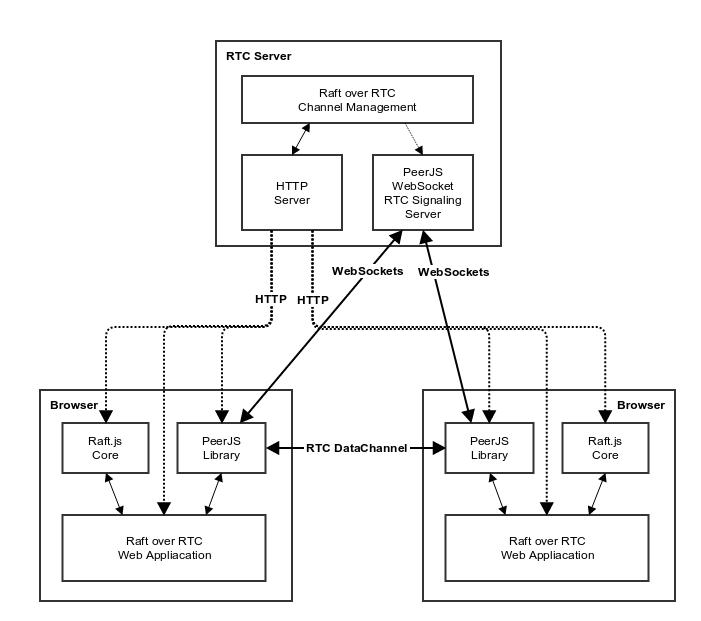
\includegraphics[width=0.45\textwidth]{imgs/raft_rtc_architecture}}
  \caption{Raft over RTC Architecture}
    \label{fig:raft_rtc_architecture}
\end{figure}

\subsection{Raft.js Core Library}

Raft.js is an implementation of the Raft algorithm in JavaScript that was created by the author of this paper \cite{raft.js}.  Raft.js is designed to run in either a browser environment or within Node.js (server-side JavaScript). Raft.js implements the Raft algorithm as described in \cite[Consensus:~Diego]{raft_thesis:ongaro14}. The core Raft algorithm is defined in the \texttt{RaftServerBase} abstract class (in \texttt{base.js}) which omits the implementation of methods with side-effects such as RPC communication, durable storage, scheduling/timeouts, or state machine command/management. The full instantiation of the class (in \texttt{rtc.js} and \texttt{chat.js}) adds state machine commands and the ability to send RPCs over the WebRTC Data Channel.

\subsection{PeerJS}

PeerJS is a project that provides a simplified abstraction for using WebRTC. The first component of PeerJS is a node.js server library that implements a WebRTC signaling server. The second component is a JavaScript library that interacts with that signaling server and also provides a simpler interface for using the WebRTC APIs.

\subsection{Signaling Server}

The file `rtc\_server.js' implements the signaling server for the Raft over WebRTC application. The server extends the PeerJS `ExpressPeerServer' object in order to provide WebRTC signaling. In addition to the WebRTC signaling function the server also serves static web resources (HTML, CSS, and JavaScript) and WebRTC channel management endpoints.

\subsection{Client}

The Raft over WebRTC chat application is a single web page (\texttt{chat.html}). When a new Raft cluster is created, the browser connects to the signaling server's new channel endpoint (Figure~\ref{fig:raft_rtc_sequence}~[1]). This endpoint causes the server to create a new channel for PeerJS signaling (Figure~\ref{fig:raft_rtc_sequence}~[2]). Once this is complete the server responds to the browser with a redirect message that contains the new channel identifier in the query parameter and ``firstServer” in the fragment identifier to indicate that this is the very first Raft cluster node (Figure~\ref{fig:raft_rtc_sequence}~[3]).

Subsequent nodes are added to the same Raft cluster by starting a new browser context (separate browser, browser window, or browser tab) and loading the same URL without the ``firstServer" fragment identifier (Figure~\ref{fig:raft_rtc_sequence}~[9]). There is a convenience link provided in the application page that opens a new browser window with a new cluster node.

When each page first loads, a PeerJS signaling connection is established with the server (Figure~\ref{fig:raft_rtc_sequence}~[6]~and~[11]). The web application also begins a periodic async polling function (\texttt{addRemoveServersAsync}) that compares the current active list of PeerJS clients to the Raft cluster membership list. If there are any differences between the two lists, then any new clients are added to the Raft cluster and missing clients are removed from the Raft cluster one at a time using the \texttt{addServer} and \texttt{removeServer} RPC calls. Servers additions are prioritized before removals in order to maximize availability \cite[Section~4.4]{raft_thesis:ongaro14}.

When an instance of the web application starts that is not a ``firstServer", the normal Raft timers are not enabled until the server receives its first RPC. The prevents the server from trying to becoming a leader before it is incorporated into the cluster by an appendEntries RPC from the true cluster leader.

\subsection{Chat Application}

\begin{figure}[!t]
  \centerline{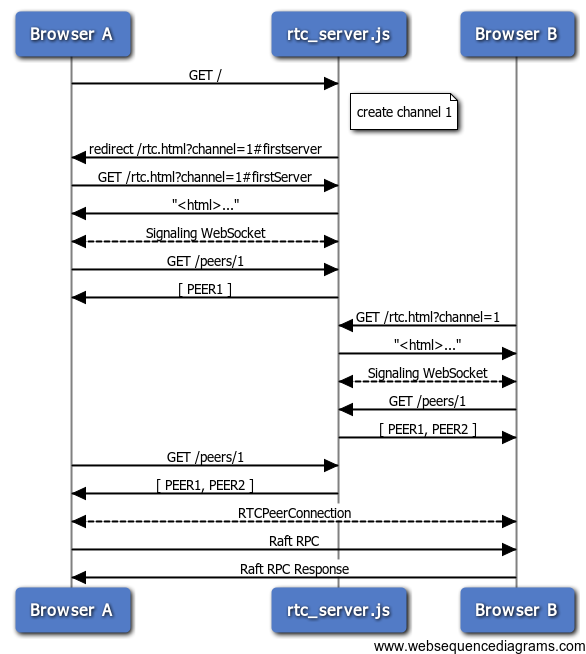
\includegraphics[width=0.45\textwidth]{imgs/raft_rtc_sequence}}
  \caption{Raft over RTC Sequence Diagram}
    \label{fig:raft_rtc_sequence}
\end{figure}

The chat application extends the basic Raft.js over WebRTC client. The chat application provides a large text area containing the chat history and a text entry field below it. When the user clicks on the \emph{Send} button (or presses enter), the current node ID is prepended to the beginning of the text line and it is added to a pending send queue and the text entry field is blanked. The chat application also extends the default set of state machine operations to add a \emph{seqAppend} operation. This is an atomic operation that is implemented as follows:

\begin{enumerate}
\item The \emph{seqAppend} operation operates on a specially structured key/value pair in the state machine map. The value of the pair is another associative map that contains a counter and list structure where the actual chat lines are accumulated. \emph{seqAppend} operations are sent with both a count and then new value to append.
\item When a \emph{seqAppend} operation is applied to the state machine and the count value in the command matches the counter in the state machine's value, then the new line in the request is added to the value list and the counter is incremented. If the count value does not match the counter then the the operation is not applied. In either case, a list is returned in the \texttt{clientRequestResponse} that contains two values: a Boolean indicating whether the \emph{seqAppend} operation succeeded and a number indicating the current value of the counter.
\item The first time the \emph{seqAppend} operation is used on a non-existent key, the structure described above is created with the counter set to 0 and the list structure is created with the single value that was passed in the \emph{seqAppend} operation.\
\item Clients that call the \emph{seqAppend} operation should check the status value in the result list. If the status is false, then the client should retry the operation. Regardless of success of failure, then client should store the current value of the counter for the next \emph{seqAppend} call or retry.
\end{enumerate}

\section{Experimental Results}

\subsection{Test Setup}

Automated testing of the Raft over WebRTC system was performed by leveraging the SlimerJS scriptable browser environment. SlimerJS enables web applications to be scripted by loading pages in a special Mozilla rendering environment called XULRunner. The XULRunner instance is directed to an X virtual frame buffer (xvfb) which provides effectively headless testing.

To simplify the execution of the tests and to make the testing infrastructure more portable, a docker container environment encapsulates and executes the SlimerJS environment. The container is built using \emph{test/Dockerfile} which is in turn derived from the ``fentas/slimerjs" docker image \cite{fentas:slimerjs}.  This custom Dockerfile was created because the upstream version of the Dockerfile used an older version of XULRunner that did not support more than 7 WebRTC clients communicating together simultaneously. This issue was discovered during initial testing.

Writing tests using SlimerJS involves creating JavaScript test programs which start a server instance and then launch a SlimerJS docker container for each node of the cluster. Each container starts a XULRunner browser instance of the Raft over WebRTC chat application. Once all the chat application nodes have connected to the test server/program, then the actual test is started across all the application nodes.

Three different tests programs/servers were created to test the basic Raft over WebRTC application. Each of the tests takes a parameter indicating the number of nodes/pages to launch. The test source files are:

\begin{enumerate}
\item \emph{test/common.js}: a module of common functions used by the other tests scripts.
\item \emph{test/test\_up.js}: launch and start an initial leader node/page, then start the rest of the nodes (if any) so that the leader will configure them into the cluster. Then test then waits for every node to be recorded (applied) into the log of every other node of the cluster. The test reports the number of milliseconds for the cluster to reach this state.
\item \emph{test/test\_kill\_nodes.js}: similar to \emph{test/test\_up.js} but once all the nodes are configured into the cluster, this script then kills the leader plus a configurable number of nodes. By default the script kills just under half the nodes of the cluster. The test then waits for a new leader to be elected and remove the dead nodes from the cluster. The test reports both the number of milliseconds for the cluster to come up and the number of milliseconds for the cluster to fully recover from the failure and evict the failed nodes.
\item \emph{test/test\_chat\_propagate.js}: similar to \emph{test/test\_up.js} but once the cluster is up, the test connects to one of the non-leader nodes and and sends a chat text line. The test then waits for the chat message to propagate to every other node's state machine. The test reports both the number of milliseconds for the cluster to come up and for the messages to propagate to every node.
\end{enumerate}

The tests were all run on a system with 8 Intel Core i7 processors running at 3.20GHz and 12 GB of main memory. The Docker image used to run the test was built using Ubuntu 12.04.5 LTS with \emph{SlimerJS} version 0.9.6, and \emph{XULRunner} version 38.0.5.

\subsection{Outcome}

\begin{figure}[!t]
    \begin{tikzpicture}
    \begin{axis}[%
        xlabel={Nodes}, ylabel={Time (seconds)},
        %xtick=data,
        xmin=0, ymin=0,
        grid=major,
        scatter/classes={%
            propagate_1_et1000={mark=x,draw=blue},
            propagate_1_et1000_average={mark=}}]
    \addplot[scatter,only marks,%
        scatter src=explicit symbolic]%
    table[meta=label] {data/propagate_1.dat};
    \addplot[scatter,%
        scatter src=explicit symbolic]%
    table[meta=label] {data/propagate_1_average.dat};
    \end{axis}
    \end{tikzpicture}
    \caption{Propagate$,$ Commit$,$ and Apply 1 Command}
    \label{fig:propagate1}
%
    \vspace{1cm}
%
    \begin{tikzpicture}
    \begin{axis}[%
        xlabel={Nodes}, ylabel={Time (seconds)},
        %xtick=data,
        xmin=0, ymin=0,
        grid=major,
        scatter/classes={%
            propagate_100_et1000={mark=x,draw=blue},
            propagate_100_et1000_average={mark=}}]
    \addplot[scatter,only marks,%
        scatter src=explicit symbolic]%
    table[meta=label] {data/propagate_100.dat};
    \addplot[scatter,%
        scatter src=explicit symbolic]%
    table[meta=label] {data/propagate_100_average.dat};
    \end{axis}
    \end{tikzpicture}
    \caption{Propagate$,$ Commit$,$ and Apply 100 Commands}
    \label{fig:propagate100}
\end{figure}

\begin{figure}[!t]
    \begin{tikzpicture}
    \begin{axis}[%
        %height=1.5\textwidth, width=1.4\textwidth,
        %width=0.45\textwidth,
        xlabel={Nodes}, ylabel={Time (seconds)},
        xmin=0, xmax=37,
        ymin=0, ymax=15,
        grid=major,
        %legend pos=outer north east,
        legend pos=north west,
        scatter/classes={%
            start_et250={mark=x,draw=magenta},
            start_et250_average={mark=,draw=red},
            %start_et250_fail={mark=x,/raw=red},
            start_et500={mark=x,draw=cyan},
            start_et500_average={mark=,draw=red},
            %start_et500_fail={mark=x,draw=red},
            start_et1000={mark=x,draw=blue},
            start_et1000_average={mark=,draw=red}}]
    \addplot[scatter,only marks,%
        scatter src=explicit symbolic]%
    table[meta=label] {data/start_et250.dat};
    \addplot[magenta,scatter,%
        scatter src=explicit symbolic]%
    table[meta=label] {data/start_et250_average.dat};

    \addplot[scatter,only marks,%
        scatter src=explicit symbolic]%
    table[meta=label] {data/start_et500.dat};
    \addplot[cyan,scatter,%
        scatter src=explicit symbolic]%
    table[meta=label] {data/start_et500_average.dat};
    %\addplot[scatter,%
    %    scatter src=explicit symbolic]%
    %table[meta=label] {data/start_et500_fail.dat};

    \addplot[scatter,only marks,%
        scatter src=explicit symbolic]%
    table[meta=label] {data/start_et1000.dat};
    \addplot[blue,scatter,%
        scatter src=explicit symbolic]%
    table[meta=label] {data/start_et1000_average.dat};

    \legend{250ms,,500ms,,1000ms,}
    \end{axis}
    \end{tikzpicture}
    \caption{Initial Cluster Activation}
    \label{fig:cluster_up}
\end{figure}

\begin{figure}[!t]
    \begin{tikzpicture}
    \begin{axis}[%
        %height=1.5\textwidth, width=1.4\textwidth,
        %width=0.45\textwidth,
        xlabel={Nodes}, ylabel={Time (seconds)},
        xmin=0, xmax=37,
        ymin=0, ymax=4.5,
        grid=major,
        %legend pos=outer north east,
        legend pos=north west,
        scatter/classes={%
            kill_1_et250={mark=x,draw=magenta},
            kill_1_et250_average={mark=,draw=red},
            %kill_1_et250_fail={mark=x,/raw=red},
            kill_1_et500={mark=x,draw=cyan},
            kill_1_et500_average={mark=,draw=red},
            %kill_1_et500_fail={mark=x,draw=red},
            kill_1_et1000={mark=x,draw=blue},
            kill_1_et1000_average={mark=,draw=red}}]
    \addplot[scatter,only marks,%
        scatter src=explicit symbolic]%
    table[meta=label] {data/kill_1_et250.dat};
    \addplot[magenta,scatter,%
        scatter src=explicit symbolic]%
    table[meta=label] {data/kill_1_et250_average.dat};

    \addplot[scatter,only marks,%
        scatter src=explicit symbolic]%
    table[meta=label] {data/kill_1_et500.dat};
    \addplot[cyan,scatter,%
        scatter src=explicit symbolic]%
    table[meta=label] {data/kill_1_et500_average.dat};
    %\addplot[scatter,%
    %    scatter src=explicit symbolic]%
    %table[meta=label] {data/kill_1_et500_fail.dat};

    \addplot[scatter,only marks,%
        scatter src=explicit symbolic]%
    table[meta=label] {data/kill_1_et1000.dat};
    \addplot[blue,scatter,%
        scatter src=explicit symbolic]%
    table[meta=label] {data/kill_1_et1000_average.dat};

    \legend{250ms,,500ms,,1000ms,}

    \end{axis}
    \end{tikzpicture}
    \caption{Recovery from Leader Failure}
    \label{fig:recovery_leader_failure}
%
    \vspace{1cm}
%
    \begin{tikzpicture}
    \begin{axis}[%
        %height=1.5\textwidth, width=1.4\textwidth,
        %width=0.45\textwidth,
        xlabel={Nodes}, ylabel={Time (seconds)},
        xmin=0, xmax=37,
        ymin=0, ymax=4.5,
        grid=major,
        %legend pos=outer north east,
        legend pos=north west,
        scatter/classes={%
            kill_half_et250={mark=x,draw=magenta},
            kill_half_et250_average={mark=,draw=red},
            %kill_half_et250_fail={mark=x,/raw=red},
            kill_half_et500={mark=x,draw=cyan},
            kill_half_et500_average={mark=,draw=red},
            %kill_half_et500_fail={mark=x,draw=red},
            kill_half_et1000={mark=x,draw=blue},
            kill_half_et1000_average={mark=,draw=red}}]
    \addplot[scatter,only marks,%
        scatter src=explicit symbolic]%
    table[meta=label] {data/kill_half_et250.dat};
    \addplot[magenta,scatter,%
        scatter src=explicit symbolic]%
    table[meta=label] {data/kill_half_et250_average.dat};

    \addplot[scatter,only marks,%
        scatter src=explicit symbolic]%
    table[meta=label] {data/kill_half_et500.dat};
    \addplot[cyan,scatter,%
        scatter src=explicit symbolic]%
    table[meta=label] {data/kill_half_et500_average.dat};
    %\addplot[scatter,%
    %    scatter src=explicit symbolic]%
    %table[meta=label] {data/kill_half_et500_fail.dat};

    \addplot[scatter,only marks,%
        scatter src=explicit symbolic]%
    table[meta=label] {data/kill_half_et1000.dat};
    \addplot[blue,scatter,%
        scatter src=explicit symbolic]%
    table[meta=label] {data/kill_half_et1000_average.dat};

    \legend{250ms,,500ms,,1000ms,}

    \end{axis}
    \end{tikzpicture}
    \caption{Recovery from Half Cluster Failure}
    \label{fig:recovery_half_failure}
\end{figure}



Figure~\ref{fig:propagate1} and Figure~\ref{fig:propagate100} show the result of running the \emph{test/wait\_chat\_propagate.js} test to determine the amount of time that a stable cluster takes to propagate, commit and apply 1 and 100 chat message commands respectively to the state machine on every cluster node using the atomic \emph{seqAppend} command. The commands are serialized which means that the previous command must be committed before the current command can be committed.  The test is complete once the last chat message command has been both committed and applied to every node of the cluster. Each test execution is shown as a blue ``x" and the black line represents the average for each cluster size.

In Figure~\ref{fig:propagate1} the time to propagate a single message to a single node of the cluster is approximately 0.1 seconds. However, this really just represents the tests scanning/checking granularity.  The time to finish propagating and committing a single message shows a slight linear slope upwards from about 0.3 seconds for a three node cluster to about 0.5 seconds for a 41 node cluster. The time to propagate 100 messages (Figure~\ref{fig:propagate100}) has a much higher slope and also appears to be non-linear.

Figure~\ref{fig:cluster_up} shows the results of running the \emph{test/test\_up.js} test to determine the amount of time that a cluster takes to start. The cluster is fully started once a leader has been elected and the leader has successfully added all the other nodes to the running configuration. Each election timer value is represented as a different color and the line represents the average value for each cluster size. The cluster startup times show a fairly linear increase as the cluster size increases. The reason that the slope varies with election timer is due to the fact that the election timer also determines the leader heartbeat value (currently set to one fifth of the election timer value). The leader heartbeat determines the frequency with which \emph{appendEntries} messages are sent from the leader to followers and is also used to propagate log entries.  This means that the rate at which log entries (and thus cluster configuration updates) can be propagated is proportional to the election timer value.

Figures \ref{fig:recovery_leader_failure} and \ref{fig:recovery_half_failure} show the results of running the \emph{test/test\_kill\_nodes.js} in both modes (kill only leader and kill just under half the nodes). Each election timer value is represented as a different color and the solid line represents the average recovery time for each cluster size. When only the leader is killed, the recovery times are constant flat regardless of cluster size. This is because after a new leader is elected, there is only a single configuration entry to propagate to the rest of the cluster (to remove the old failed leader). One interesting thing to note is that with a 1000ms timer, the 3 node cluster is actually the most inefficient size because the average time until a leader election starts is inversely proportional to cluster size so the delay until an election happens is a significant contributor to the three node cluster with 1000ms timer. With a larger cluster or shorter election timer, the contribution of election delay is not noticeable. The recovery from almost half the nodes failing is not flat because the amount of configuration information that needs to be propagated is proportional to the size of the cluster.

\section{Future Work}

One of the useful outcomes of this project was that it brought to light many areas where further study of Raft, WebRTC, and Raft over WebRTC should be pursued. Here are some interesting areas for further exploration:

\begin{enumerate}
\item Explore models for dynamically adjusting Raft timeout values to account for changing network and browser conditions.
\item Explore alternate WebRTC transport modes for relaxing ordering constraints and delivery guarantees. Since the Raft protocol is tolerant of out-of-order and dropped messages, it is possible that Raft over WebRTC could be more efficient with one or both of these constraints relaxed.
\item Test the survivability of the cluster when the signaling server becomes completely unresponsive or very slow.
\item Test larger scale deployments spanning larger and more diverse network domains. Characterize the factors that affect and limit scalability.
\item Explore models for timing out and automatically removing nodes when they become unresponsive without needing to be notified by the signaling server that the nodes have disconnected.
\item Consider extensions to the Raft protocol that enable slow leaders to be proactively detected so that a more capable node (network, CPU, etc) can be elected. This would help address that background page/tag throttling of modern browsers.
\item Explore models that allow for a combination of strict shared state and high performance bulk data such as media or object blobs.
\end{enumerate}


\section{Conclusion}

The ability to create distributed applications that minimize dependence on centralized infrastructure is important for many use cases. The combination of the Raft distributed consensus algorithm with the WebRTC communication protocol enables a powerful middleware system for building powerful distributed browser-to-browser applications. The Raft over WebRTC middleware system is able to easily scale to at least 35 node clusters and that it can quickly recover from multiple node failures. Further study may show that a dynamically tuned election timer that accounts for communication latency would allow the cluster size to be scaled well beyond 35 nodes.


\section*{Acknowledgments}

I would like to thank my academic supervisor, David Levine, for his excellent input and oversight of this project. I would also like to thank Diego Ongaro for his amazing work on the Raft protocol and paper which made implementing a Raft implementation a pleasure.  There are too many people involved in the creation and standardization of WebRTC but I would like to thank them for their tireless work to make browser-to-browser communication possible. Last but not least, I would like to thank my family for putting up with the long nights and weekends I spent on this project. Thanks!

\bibliographystyle{./IEEEtranBST2/IEEEtran}
\bibliography{./references/ietf,./references/w3c,./references/raft,./references/other}

\end{document}

